\documentclass[11pt]{article}

\usepackage[margin=1in]{geometry}
\usepackage{times}
\usepackage{helvet}
\usepackage{courier}
\usepackage{array}
\usepackage{amsmath}
\usepackage{amsthm}
\usepackage{amsbsy}
\usepackage{amssymb}
\newtheorem{definition}{Definition}
\usepackage{graphicx}
\usepackage[dvipsnames]{xcolor}
\usepackage{mathtools}
\usepackage{nicefrac}
\usepackage{bm}
\usepackage{enumitem}
\usepackage{mpemath}
\usepackage{tcolorbox}
\usepackage[capitalize,noabbrev]{cleveref}
\usepackage{theoremref}
\usepackage{algorithm}
\usepackage{algpseudocode}
\usepackage{tikz}
\renewcommand{\algorithmicrequire}{\textbf{Input:}}
\renewcommand{\algorithmicensure}{\textbf{Output:}}
%===================================
\newtheorem{theorem}{Theorem}
\newtheorem{lemma}{Lemma} 
\newtheorem{proposition}{Proposition}
\newtheorem{assumption}{Assumption} 

\newcommand{\mm}[1]{\textcolor{blue}{[#1]}}
\newcommand{\gersi}[1]{\textcolor{red}{[#1]}}
\newcommand{\s}[1]{\mathcal{#1}}

\setlength{\parskip}{3mm plus 1mm minus 1mm}
\setlength{\parindent}{0pt}

\title{Robust Inverse Reinforcement Learning Without Homogeneous Trajectories}
\author{Gersi Doko, Marek Petrik}

\begin{document}

\maketitle

\begin{abstract}
	\begin{enumerate}
		\item What is the problem we address and what is the limitation of earlier work.
		\item Not enough data to estimate occupancy frequencies reliably, estimation
		      error, a lot of data is needed to reliably learn.
		\item Expert demonstrators may bias demonstrations to most informative states to
		      demonstrate challenging or difficult states leading to an incorrect estimate
		\item This paper proposes this kind of an approach. How is this new and better.
	\end{enumerate}
\end{abstract}

% \section{TODO}
% \begin{enumerate}
%   \item Formalize what guarantees we can make about states we have not seen in $\mathcal{D}$
%   \item Continuous state space
% \end{enumerate}

\section{Introduction}
% \begin{enumerate}
%   \item What problem exactly are we trying to solve
%   \item why is it important
%   \item why is it hard
%   \item what is our main insight
%   \item contribution section 
%   \item Start with the point of the paper early.
%   \item One idea per paragraph
%   \item open with a statement about the paragraph
% \end{enumerate}

The objective of Inverse Reinforcement Learning (IRL) is to learn a policy given expert demonstrations~\cite{abbeel2004, chang2021mitigating}
\mm{good to cite a broder range of work including some recent papers}. 
Note that given the true reward function this problem would be equivalent to solving a Markov Decision Process (MDP)~\cite{PUTERMAN}.
Like in the work by Abbeel et al. we assume that the true reward function can be written as a linear combination of the features $\Phi$ which are known. 
The general formulation of the IRL problem is\dots
\begin{equation} \label{eq:IRL_formulation}
	\min_{\pi \in \Pi} \max_{r \in \mathcal{R}} (\rho(\pi_e, r) - \rho(\pi, r)),
\end{equation}
where $\Pi$ is the set of all policies with $\pi_e \in \Pi$, $\mathcal{R}$ is the set of all reward functions, and $\rho$ is the return of a policy given some reward function. This setting is useful for domains where the reward function is hard to define, but features and demonstrations are available. Such domains include robotics, medicine, and autonomous driving. We will focus on the robust IRL problem, where there is an inner maximization over $\Pi$, see \cref{sec:optimization-formulation}.

Most prior work on IRL suffers from a major limitation. Namely, the problem of covariate shift. Covariate shift occurs when the training data follows a different distribution than the test data. Put in context, the state distribution of the behavior policy $d_b$ is different from the state distribution of the expert policy $d_e$. Our goal is to recover the expert policy $\pi_e$ even when such a distinction exists between the behavior policy and the expert.

Our focus is in the offline setting where we are given a dataset which contains states and actions generated by the expert. This setting does not allow querying the expert, and thus is much harder than the online setting. To our knowledge no work has been published which guarantees a solution to the covariate shift problem in the model based offline setting.

We make three main contributions in this work. First, we present a new approach to overcoming covariate shift in the model based offline setting. Second, we provide a strong analysis which guarantees performance, both in data efficiency and in return. Third, we show how our method can be applied when the transition dynamics are unknown, and for continuous state spaces.

The main idea of our approach is to represent the IRL problem as a robust optimization over the policy space and simplify it to a linear program. To this end we employ Chebyshev approximation, and constraint generation. For tabular settings the resulting LP can be solved very efficiently using a commercial solver. For non-tabular MDPs we describe an extension to our method \gersi{which is currently under development}.

\paragraph{Notation} $\Delta^{\mathcal{S}}$ is the simplex over the elements of the set $\mathcal{S}$. $\mathcal{A}^{\mathcal{B}}$ represents the set of all functions from $\mathcal{B}$ to $\mathcal{A}$. Similarly, $\Real^N$ where $N$ is a natural number, represents the $N$ dimensional vector space.  If $\mathcal{B}$ is an index set such as $\mathcal{B} = \left\{ 1, \ldots , B \right\}$, we will use $\Real^{\mathcal{B}}$ interchangeably as a space of functions and a space of $B$-dimensional
vectors.

\section{Preliminaries}\label{sec:preliminaries}

Here we provide a brief introduction to MDPs as well as the IRL problem. We will use this machinery to build up our solution in the following sections.
This introduction is not meant to be exhaustive, but rather to provide the reader with the necessary background to understand the rest of the paper.
Much of the MDP material comes from~\cite{PUTERMAN}. For a more in-depth treatment of the IRL setting we refer the reader to~\cite{abbeel2004}.

\paragraph{MDP}
The domain is modeled as a Markov Decision Process with a finite number of states $\mathcal{S} = \left\{ 1, \dots , S \right\}$ and a finite number of actions $\mathcal{A} = \left\{ 1, \dots , A \right\}$. The transition probability function $p\colon \mathcal{S} \times \mathcal{A} \to \Delta^{\mathcal{S}}$ is known. The true reward function $r\opt \colon \mathcal{S} \times \mathcal{A} \to \Real$ is unknown, and we learn it from data. The set of possible reward functions is denoted as $\mathcal{R} \subseteq \Real^{\mathcal{S} \times \mathcal{A}}$. The set of deterministic policies is $\Pi_D= \mathcal{A}^{\mathcal{S}}$ and the set of randomized policies is $\Pi_R = {\left(\Delta^{\mathcal{A}}\right)}^{\mathcal{S}}$. The set of all policies is $\Pi = \Pi_R \cup \Pi_D$.

We assume the $\gamma$-discounted infinite horizon objective with $\gamma \in [0,1)$. 
The infinite-horizon discounted return of a policy $\pi \in \Pi$ and a reward $r \in \mathcal{R}$ is denoted by $\rho(\pi, r)$. 
An important fact that we will need to develop our algorithms is the well-known connection between the occupancy frequencies and policies. 
For any policy $\pi\in\Pi_R$ and an initial distribution $p_0\in \Delta^{\mathcal{S}}$, there exists an occupancy frequency $u\in \Real^{\mathcal{S}\mathcal{A}}$. 
The space of occupancy frequencies for all $\pi\in \Pi_R$ and a fixed initial distribution $p_0$ is denoted as $\mathcal{U}$
and is discussed in depth in~\cite{PUTERMAN}:
\[
	\mathcal{U} = \left\{ u\in \Real^{SA}_{+} \mid \sum_{a\in \mathcal{A}} (I - \gamma\cdot P\tr_a) u(\cdot, a) = p_0 \right\}~.
\]

\paragraph{IRL}
Assume that the expert follows a policy $\pi_e$. And that we follow a distribution $d_b \subset \Delta^{\mathcal{S}}$
which produces a dataset of non-homogeneous (unordered / non-sequential)
trajectories $\mathcal{D} = {(s_i \sim d_b, \pi_e(s_i))}_{i=1}^D$. In this work, we aim
to develop a robust algorithm which can learn a reward function that is
consistent with the expert when our given demonstrations, $\mathcal{D}$,
demonstrate actions in a small subset of the set $\mathcal{S}$ in a
non-sequential manner.

To enable the generalization of the learned reward function, we assume to be given a feature function $\phi: \mathcal{S} \times \mathcal{A}\to \Real^k$. That is, for each state and action there are $k$ features which represent some heuristic regarding the respective state and action. Through an arbitrary ordering of states, we can represent our features with a feature matrix $\Phi \subset \Real^{SA\times k}$. Note that while any ordering of state, action pairs is sufficient, in this paper we will assume the following without loss of generality\dots
\begin{enumerate}
	\item We are given some ordering of states, $\mathcal{S} = \{ s_1, s_2, \dots, s_i \}$
	\item We are given some ordering of actions, $\mathcal{A} = \{ a_1, a_2, \dots, a_j \}$.
	\item When vectors or matrices are indexed by a state, action pair $(s,a)$; they are assumed to iterate over
	      states first then actions.
\end{enumerate}

In this paper we investigate linear reward function approximation, that is we seek to find a $w \in \mathcal{W} \subseteq \Real^k$ s.t. $r\opt(s,a) = w\tr
	\phi(s,a)$ $\forall s \in \mathcal{S}$, $\forall a \in \mathcal{A}$. To
prevent hyper-scaling of our learned parameter, $w$, we restrict it by
ensuring its norm is upper bounded by a constant. We consider the following
forms of $w$ regularization; $\mathcal{R}_{1+} = \left\{ w \in \Real^K_+
	\mid \| w \|_1 \le 1 \right\}$ and $\mathcal{R}_2 = \left\{ w\in \Real^K
	\mid  \|w \|_2 \le 1 \right\}$.

\gersi{We don't talk about R2 in this paper should we keep it here?}

\section{Optimization Formulation}\label{sec:optimization-formulation}
Now we illustrate the robust IRL learning problem as an optimization problem over the policy and reward space. Then we simplify it using occupancy frequencies
and the fact that the reward function is linearly realizable by $\Phi$. This allows us in the following section to formulate the problem as a linear program.

Recall the IRL objective\dots

\begin{equation}
	\min_{\pi \in \Pi} \max_{r \in \mathcal{R}} (\rho(\pi_e, r) - \rho(\pi, r)),
\end{equation}

We only observe $\pi_e \in \Pi_D$ through its demonstrations $\mathcal{D}$. Therefore, we define a set of randomized policies which are consistent with $\pi_e$.

\begin{equation} \label{eq:consistent-policies}
	\Pi_R(\mathcal{D}) = \left\{ \pi \in \Pi_R \mid \pi(s,a) = 1, \, \forall (s,a) \in \mathcal{D} \right\}~.
\end{equation}

Note that if a randomized policy were used to generate the demonstrations in
$\mathcal{D}$, then the set $\Pi(\mathcal{D})$ may be empty. We want to be robust with respect to the policies which mimic $\pi_e$. 
We now turn to the robust IRL problem as an optimization which fulfills our needs\dots

\begin{equation}
	\label{eq:robust_IRL_formulation}
	\min_{\pi \in \Pi} \max_{r \in \mathcal{R}} \max_{\pi_e \in \Pi_{R}(D)} \rho(\pi_e, r) - \rho(\pi, r)
\end{equation}

\mm{We allow for randomized policies in~\eqref{eq:consistent-policies}, but I
	think that we can argue then it does not matter because the optimization problem
	will always find a deterministic policy.}
\gersi{Will it always find a deterministic policy?}

We will find it useful to define the set of consistent occupancy frequencies $\Upsilon(\mathcal{D})$, as our goal is to introduce an LP to solve
the robust IRL problem.

Let $c \in \Real^{SA}$ such that $c(s,a) = 1$ if $(s,a) \notin \mathcal{D}$ and $(s, \cdot) \in \mathcal{D}$, $c(s,a)  = 0$ otherwise.

\begin{equation}\label{eq:consistent-occupancies}
	\Upsilon(\mathcal{D}) = \left\{ u \in \mathcal{U} \mid c\tr u = 0  \right\}~.
\end{equation}

This set constrains occupancy frequencies to 0 only for the state-action pairs in which the state was observed, but the action was not. 
This constraint penalizes policies which are inconsistent with the demonstrations.

\begin{proposition}\label{prop:convexity_of_Upsilon}
	$\Upsilon$ is convex, closed, and polyhedral. 
\end{proposition}

\begin{proof}
	$\mathcal{U}$ is a union of hyperplanes therefore $\Upsilon$ is a union of
	closed hyperplanes. Any union of closed hyperplanes is convex and closed~\cite{boyd_convex_optimization} (2.2.1).
	$\Upsilon$ is polyhedral by the dual LP formulation of~\cite{PUTERMAN} (6.9.2).
\end{proof}

The following lemma states the correctness of the construction of the occupancy
frequencies in~\eqref{eq:consistent-occupancies}. In particular, it shows that
$\Upsilon$ is exactly the set of occupancy frequencies that are consistent with the
dataset. And these occupancy frequencies correspond to randomized policies that are also consistent with the dataset.

\begin{lemma}\label{lemma:occ_freq_matching}
	Assume that $\mathcal{D}$ is the set of trajectories generated by some unknown deterministic policy $\pi_e \in \Pi_D$. Then
	\[
		u \in \Upsilon(\mathcal{D})  \quad \Leftrightarrow \quad  \exists \pi \in \Pi_R(\mathcal{D}), \, u = u^{\pi}~,
	\]
	for each $\pi \in \Pi$ where $u^{\pi}$ is the occupancy frequency of the policy $\pi$.
\end{lemma}
\begin{proof}
	Included in the appendix for brevity.
\end{proof}

Observe that given Lemma~\ref{lemma:occ_freq_matching} maximizing over the policy space is equivalent to maximizing over the occupancy frequency space.
Also note that $\rho(\pi,r) = u_{\pi}^T r$ where $u_{\pi}$ is the occupancy frequency of policy $\pi$. This allows us to simplify~\eqref{eq:robust_IRL_formulation} as follows\dots

\begin{equation}
	\min_{u \in \mathcal{U}} \max_{r \in \mathcal{R}} \max_{v \in \Upsilon} v^T r - u^T r
\end{equation}

Next observe that maximizing over $r \in \mathcal{R}$ is equivalent to maximizing over $w \in \mathcal{W}$ since we assume that $r^* = \Phi w^*$.

\begin{equation}\label{eq:primal-robust-irl}
	\min_{u \in \mathcal{U}} \max_{w \in \mathcal{W}} \max_{v \in \Upsilon} (v - u)^T \Phi w
\end{equation}

From~\cite{PUTERMAN} it is known that we can convert between policies and occupancy frequencies as follows\dots

\begin{equation}\label{eq:policy-construction}
	\pi(s, a) = \frac{u^{\pi}(s,a)}{\sum_{a` \in \mathcal{A}} u^{\pi}(s,a`)}
\end{equation}

The following theorem shows the correctness of our approach.

\begin{theorem}\label{thrm:chebeyshev-regret}
	Suppose that $\hat{\pi}$ has an occupancy frequency $u_{\hat{\pi}} \in \arg\min_{u \in \mathcal{U}} \max_{w \in \mathcal{W}} \max_{v \in \Upsilon} (v - u)^T \Phi w$.
	Then $\hat{\pi}$ minimizes the worst-case regret with respect to the worst-case
	policy consistent with the demonstrations $\mathcal{D}$. That is,
	\[
		\max_{r\in \mathcal{R}} \max_{\pi \in \Pi_{R}(\mathcal{D})} \left(\rho(\pi, r) - \rho(\hat{\pi}, r)\right)
		\; \le\;
		\max_{r\in \mathcal{R}} \max_{\pi \in \Pi_{R}(\mathcal{D})} \left(\rho(\pi, r) - \rho(\pi', r)\right), \quad  \forall \pi' \in \Pi~,
	\]
\end{theorem}

\begin{proof}
	Included in the appendix for brevity.
\end{proof}

\mm{Maybe it would be nice to give some name to the regret with respect to the worst-case consistent policy.}

When we consider $\mathcal{W} = \Real_{1+}$ equation~\eqref{eq:primal-robust-irl} can be simplified using the definition of the dual norm on the maximization
over $w$. For simplicity, the definition of the dual norm is included here. For $\mathcal{W}$ bounded by some $L_p$ ball $\max_{w \in \mathcal{W}} \Phi w = ||\Phi||_*$.
The particular reader should note that indeed~\eqref{eq:primal-robust-irl} can be written as\dots

\begin{equation}
	\min_{u \in \mathcal{U}} \max_{v \in \Upsilon} \max_{w \in \mathcal{W}} {(v - u)}^T \Phi w
\end{equation}

\begin{equation}
	\label{eq:robust_IRL_formulation_L1}
	\min_{u \in \mathcal{U}} \max_{v \in \Upsilon} ||\Phi\tr (v - u)||_*
\end{equation}

The set $\mathcal{U}$ is convex by the dual LP in~\cite{PUTERMAN} (6.9.2).
Likewise, by Proposition~\ref{prop:convexity_of_Upsilon} $\Upsilon$ is convex.
Finally, any norm on $\Real^K$ is convex~\cite{boyd_convex_optimization} (3.1.5).
Therefore, the optimization in~\eqref{eq:robust_IRL_formulation_L1} is a convex
optimization problem. In the convex optimization literature,
~\eqref{eq:robust_IRL_formulation_L1} is a problem of finding the largest minimum
distance between the edges of polytopes $\mathcal{U}$ and $\Upsilon$. Also known as the Chebyshev center of $\Upsilon$ with respect to $\mathcal{U}$.
This problem is known to be NP-hard except for certain cases \gersi{We need a
	citation for this because I don't buy it}.\gersi{ Make sure to reference the analysis section when you add the discussion there.}

Since $\mathcal{W}$ is bounded by the $L_1$ norm, its dual is the $L_\infty$ norm. The extreme points of the above
optimization problem can be enumerated precisely as follows.
This is done to reduce the optimization problem and improve efficiency.

\begin{equation}
	\label{eq:extreme_points_of_the_IRL_Formulation}
	\min_{u \in \mathcal{U}} \max_{v \in \Upsilon} \max_{i \in 1:k} \max|(v - u)\tr \Phi_i|
\end{equation}

The equation in~\eqref{eq:extreme_points_of_the_IRL_Formulation} can be seen as
finding the feature-vector which points in the same SA-dimensional direction as
the difference between our estimated occupancy frequency $u$ and the experts
$v$. For those familiar with prior works done by Syed and Schapire~\cite{Syed2008} this is very similar to LPAL and MWAL. 
However, we show that our formulation is more general and can recover the expert exactly in particular cases.

\section{Solving the Optimization Formulation}
\begin{enumerate}
	\item Solve the above equation
	\item Can we show that the problem is NP hard for some choices of the set $\mathcal{R}$? \mm{
		      Some relevant papers are:~\cite{Wu2013,Eldar2008}
	      }
\end{enumerate}

Recall the definition of $\Phi \in \Real^{SA \times K}$ given some arbitrary ordering on $(s,a)$ pairs.
\begin{center}

	\[\*\Phi\tr \;=\; \begin{bmatrix}
			- & \phi_1\tr & - \\
			- & \phi_2\tr & - \\
			- & \vdots    & - \\
			- & \phi_K\tr & -
		\end{bmatrix}\]

	Where $\phi_n = [\phi_n(s,a)\;\;\forall s,a \in S \times A]$ represents the n'th feature evaluated on each $(s,a)$ pair.
\end{center}

We apply a technique called Chebyshev Approximation~\cite{boyd_convex_optimization}(6.1) to equation~\eqref{eq:extreme_points_of_the_IRL_Formulation}.
This step can also be seen as writing~\eqref{eq:extreme_points_of_the_IRL_Formulation} in epigraph form.

\begin{equation}
	\begin{mprog}
		\minimize{u \in \mathcal{U}, \sigma \in \Real} \sigma
		\stc \max_{v \in \Upsilon} |(v - u)\tr \Phi_i| \leq \sigma
		\cs i \in 1 \dots k
	\end{mprog}
\end{equation}

After expanding the absolute value is equivalent to\dots

\begin{equation}
	\begin{mprog}
		\minimize{u \in \mathcal{U}, \sigma \in \Real} \sigma
		\stc \max_{v \in \Upsilon} (v - u)\tr \Phi_i \leq \sigma
		\cs \max_{v \in \Upsilon} -(v - u)\tr \Phi_i \leq \sigma
		\cs i \in 1 \dots k
	\end{mprog}
\end{equation}

In order to make the above problem more easily solvable, let us take the dual of the first inner maximization problem. That is\dots

\begin{equation}
	\begin{mprog}
		\maximize{v \in \Upsilon} (v - u)\tr \Phi_i
		\cs i \in 1\dots k
	\end{mprog}
\end{equation}

Notice in order to get this into an LP form we need to take the convex set $\Upsilon$ and construct a linear constraint which encapsulates
what it means for an element $v \in \Real_+^{SA}$ to be in the set $\Upsilon$. 
Luckily this is easy to do as $\Upsilon$ is defined as a linear constraint on $\mathcal{U}$.
For the sake of simplicity suppose that we consider one fixed $\Phi_i$, and omit the optimization over all $i \in 1\dots k$ for the duration
of the dual derivation. But do keep in mind, each feature vector gets its own dual variable.

\begin{equation}
	\label{eq:primal_IRL_problem}
	\begin{mprog}
		\maximize{v \in \Real_+^{SA}} (v - u)\tr \Phi_i
		\stc c\tr v = 0
		\cs \sum_{a \in \mathcal{A}}(I - \gamma P_a\tr)v(\cdot, a) = p_0
	\end{mprog}
\end{equation}

\begin{equation}
	L(v, \alpha, \beta) = (v - u)\tr \Phi_i + \alpha c\tr v
	+ \beta\tr (\sum_{a \in \mathcal{A}}(I - \gamma P_a\tr)v(\cdot, a) - p_0)
\end{equation}

Writing the summation as a matrix vector multiplication we have.

\[\*A \;=\; \begin{bmatrix}
		- & (I - \gamma P_1) & - \\
		- & (I - \gamma P_2) & - \\
		- & \vdots           & - \\
		- & (I - \gamma P_a) & - \\
	\end{bmatrix}\;\in\; \Real^{SA\times S}\]

\begin{equation}
	\label{eq:rewrite_U_constraint}
	L(v, \alpha, \beta) = (v - u)\tr \Phi_i + \alpha c\tr v
	+ \beta\tr (A\tr v - p_0)
\end{equation}

Notice that we assume that the vector $v \in \Real^{SA}$ iterates over states first before iterating over actions.

\begin{equation}
	g(\alpha, \beta) = \sup_{v\geq 0} L(v, \alpha, \beta)
\end{equation}

\begin{equation}
	g(\alpha, \beta) = -u\tr \Phi_i - \beta\tr p_0 + \sup_{v\geq 0} (v\tr \Phi_i + \alpha c\tr v + \beta\tr A\tr v)
\end{equation}

\begin{equation}
	g(\alpha, \beta) = -u\tr \Phi_i - \beta\tr p_0 + \sup_{v \geq 0} (\Phi_i\tr + \alpha c\tr + \beta\tr A\tr)v
\end{equation}

Notice that the quantity in the parentheses is linear in $v$, and linear functions are
bounded above if and only if their coefficient is 0.
Therefore, $g(\alpha, \beta) = \infty$ except for when $\Phi_i + \alpha c + A\beta \leq 0$ in which case
$g(\alpha, \beta) = -u\tr \Phi_i - \beta\tr p_0$.

Now we are ready to define the dual of~\eqref{eq:primal_IRL_problem}.
Given that $g(\alpha, \beta)$ is an upper bound on the optimal value of~\eqref{eq:primal_IRL_problem} for feasible $v$, we wish to minimize it.

\begin{equation}
	\begin{mprog}
		\minimize{\alpha \in \Real, \beta \in \Real^{S}} -u\tr \Phi_i - \beta\tr p_0
		\stc \Phi_i + \alpha c + A\beta \leq 0
	\end{mprog}
\end{equation}

Recall the formulation of the Chebyshev Center.
\begin{equation}
	\begin{mprog}
		\minimize{u \in \mathcal{U}, \sigma \in \Real} \sigma
		\stc \max_{v \in \Upsilon} (v - u)\tr \Phi_i \leq \sigma
		\cs \max_{v \in \Upsilon} -(v - u)\tr \Phi_i \leq \sigma
		\cs i \in 1 \dots k
	\end{mprog}
\end{equation}

Now derive a similar result for the second maximization using the same method as above and substitute.
Recall that each feature-vector has its own unique dual variables.

\begin{equation}
	\begin{mprog}
		\minimize{u\in\mathcal{U}, \sigma\in\Real} \sigma
		\stc \min_{\alpha_i \in \Real, \beta_i \in \Real^{S}} -u\tr \Phi_i - \beta_i\tr p_0 \leq \sigma
		\cs \Phi_i + \alpha_i c + A \beta_i \leq 0
		\cs \min_{\hat{\alpha}_i \in \Real, \hat{\beta}_i \in \Real^{S}} u\tr \Phi_i - \hat{\beta}_i\tr p_0 \leq \sigma
		\cs -\Phi_i + \hat{\alpha}_i c + A \hat{\beta}_i \leq 0
		\cs i \in 1 \dots k
	\end{mprog}
\end{equation}

\begin{equation}
	\begin{mprog}
		\label{eq:semi_fininished_LP}
		\minimize{u\in\mathcal{U}, \sigma, \alpha_i, \hat{\alpha}_i \in \Real, \beta_i, \hat{\beta}_i \in \Real^{S}} \sigma
		\stc -u\tr \Phi_i - \beta_i\tr p_0 \leq \sigma
		\cs u\tr \Phi_i - \hat{\beta}_i\tr p_0 \leq \sigma
		\cs \Phi_i + \alpha_i c + A \beta_i \leq 0
		\cs -\Phi_i + \hat{\alpha}_i c + A \hat{\beta}_i \leq 0
		\cs i \in 1 \dots k
	\end{mprog}
\end{equation}

And now for the final push, notice that~\eqref{eq:semi_fininished_LP} is not an LP,
because of the nonlinear (yet convex) minimization over $u\in\mathcal{U}$. To remedy this notice
how we re-wrote the definition of $\mathcal{U}$ in~\eqref{eq:rewrite_U_constraint}. This leads us to the
LP formulation of the Chebyshev Center\dots
\gersi{TODO go back and explain why the $A^{T}v$ constraint makes sense}

\begin{equation}
	\begin{mprog}
		\minimize{\sigma, \alpha_i, \hat{\alpha}_i \in \Real, \beta_i, \hat{\beta}_i \in \Real^{S}, u \in \Real^{SA}} \sigma
		\stc -u\tr \Phi_i - \beta_i\tr p_0 \leq \sigma
		\cs u\tr \Phi_i - \hat{\beta}_i\tr p_0 \leq \sigma
		\cs \Phi_i + \alpha_i c + A \beta_i \leq 0
		\cs -\Phi_i + \hat{\alpha}_i c + A \hat{\beta}_i \leq 0
		\cs i \in 1 \dots k
		\cs A\tr u = p_0
		\cs u \geq 0
	\end{mprog}
\end{equation}

\section{Analysis}

\mm{Things to show:
	\begin{enumerate}
		\item When each state is present in the dataset, then we can compute a policy
		      that has zero worst-case regret
		\item What if there is one state that we have not seen, can we bound the
		      regret then?
	\end{enumerate}
}
\begin{enumerate}
	\item By this point our main algorithm should be defined, in this section we
	      try and show our method is better than occupancy frequency matching.
	\item We set up the theoretical bounds of our method to empirically show them
	      in the next section.
\end{enumerate}

Define $\mathcal{D}_S$ to be the set of all states that have been observed in expert's trajectories:
\[
	\mathcal{D}_S  = \left\{ s\in \mathcal{S} \; \mid \; \exists\; a\in \mathcal{A}, \; (s,a) \in \mathcal{D} \right\}~.
\]

\begin{proposition}
	If $\mathcal{D}_\mathcal{S} = \mathcal{S}$ then $|\Upsilon(\mathcal{D})| = 1$
	and $u \in \Upsilon(\mathcal{D}) \Rightarrow u = u^{\pi_e}$.
\end{proposition}

\begin{proof}
	Given $\mathcal{D}_\mathcal{S} = \mathcal{S}$ then $|\Pi_R(\mathcal{D})| = 1$
	because there can only be one policy consistent with the demonstration
	$\mathcal{D}$ since every state was mapped to an action by $\pi_e \in \Pi_D$
	which generated $\mathcal{D}$. Therefore, by Lemma 1, $u^\pi$ for $\pi \in
		\Pi_R(\mathcal{D})$ is the only occupancy frequency consistent with the
	demonstration, and thus $|\Upsilon(\mathcal{D})| = 1$. By the above
	statements, $u \in \Upsilon(\mathcal{D}) \Rightarrow u = u^{\pi_e}$.
\end{proof}

\paragraph{Limitations of ROIL}
Consider the following deterministic MDP, where $S = \{s_1, s_2, s_3\}$, $A = \{a_1, a_2\}$, $p_0 = [1,0,0]$,
and $\Phi = r^* = [0,0,1,1,-1,-1]$:
\begin{center}
	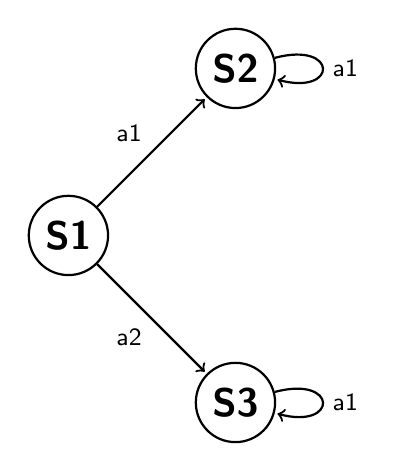
\begin{tikzpicture}[->,shorten >=1pt,auto,node distance=3cm,
			thick,main node/.style={circle,draw,font=\sffamily\Large\bfseries}]

		\node[main node] (1) {S1};
		\node[main node] (2) [above right of=1] {S2};
		\node[main node] (3) [below right of=1] {S3};

		\path[every node/.style={font=\sffamily\small}]
		(1) edge node [above left] {a1} (2)
		edge node [below left] {a2} (3)
		(2) edge [loop right] node {a1} (2)
		(3) edge [loop right] node {a1} (3);
	\end{tikzpicture}
\end{center}

Solving this MDP yields $u_e = [1,0,\frac{\gamma}{1-\gamma},0,0,0]$, however ROIL fails to find this solution for some datasets.
While other less involved methods like LPAL~\cite{Syed2008} successfully recover $u_e$ no matter the dataset. Take for example
$D = [(s_2, a_1)]$, this causes ROIL to find $u = [\frac{1}{2},\frac{1}{2},\frac{\gamma}{2(1-\gamma)},0,\frac{\gamma}{2(1-\gamma)},0]$.
This example exposes two downsides of ROIL. Firstly, the pessimistic nature of ROIL, it assumes that the expert is trying to maximize the worst-case reward, 
and thus its solution randomizes among the actions in the first state. Secondly, ROIL cannot take advantage the number of times that a state action pair is visited,
and therefore what makes a dataset good for LPAL and other occpancy matching methods is not necessarily good for ROIL.

\section{Experimental Results}
\begin{enumerate}
	\item Discuss our experiments using the above defined algorithms.
	\item Discuss whether our algorithm meets its analytical results.
	\item Demonstrate its performance on up-to-date sandboxes.
\end{enumerate}

\section{Conclusion}
\begin{enumerate}
	\item Restate the main idea that lead us to this problems' solution.
	\item Restate the performance of our method.
	\item Outline where these ideas could be applied in the future.
\end{enumerate}

\bibliography{irl.bib}
\bibliographystyle{plain}

\section{Appendix}
\begin{enumerate}
	\item Prove theorems here to give the above sections brevity
	\item only prove theorems in the above sections if absolutely instrumental
	      to the paper
\end{enumerate}

\paragraph{Proof of Lemma~\ref{lemma:occ_freq_matching}}
Assume that $\mathcal{D}$ is the set of trajectories generated by some unknown deterministic policy $\pi_e \in \Pi_D$. Then
\[
	u \in \Upsilon (\mathcal{D})  \quad \Leftrightarrow \quad  \exists \pi \in \Pi_R(\mathcal{D}), \, u = u^{\pi}~,
\]
for each $\pi \in \Pi$ where $u^{\pi}$ is the occupancy frequency of the policy $\pi$.
\begin{proof}
	To do this, we use the policy to occupancy frequency correspondence~\cite{PUTERMAN}.
	\[\forall \pi \in \Pi \,\,\,\, u^\pi(s,a) = \pi(a|s)\sum_{a`}{u^\pi(s,a`)}\]

	Case 1: Prove $u \in \Upsilon (\mathcal{D})  \quad \Rightarrow \quad  \exists
		\pi \in \Pi_R(\mathcal{D}), \, u = u^{\pi}$,

	Given $u \in \Upsilon (\mathcal{D})\,\,$ constructing policy $\pi$ from
	occupancy frequency $u$ via the policy occupancy correspondence we have\dots

	\[\pi(a|s) = \frac{u(s,a)}{\sum_{a`}u(s,a`)}\]

	Since $u \in \Upsilon (\mathcal{D})$, $u\tr c = 0$ for some $c \in \Real^{SA}$ such that 
	$c(s,a) = 1$ if $(s,\cdot) \in \mathcal{D}, (s,a) \notin \mathcal{D}$ and $c(s,a) = 0$ otherwise. 
	Therefore, for states $s$ where $(s,\cdot) \in \mathcal{D}$ we have $u(s,a) = 0$ for all $a \not= \pi_e(s)$.
	Only one action for that state will be non-zero, therefore for observed states we have $\pi(a|s) = 1$.

	Case 2: Prove $\pi \in \Pi_R(\mathcal{D}) \quad \Rightarrow \quad  u^\pi \in
		\Upsilon (\mathcal{D})$

	Given that $\pi \in \Pi_R(\mathcal{D})$, $\pi(a|s) = 1$ for all $(s,a) \in \mathcal{D}$. Therefore, for observed states $s$, $u(s,a) = 0$ for all $a \not= \pi_e(s)$
	since $u(s,a) = \pi(a|s)\sum_{a`}{u^\pi(s,a`)}$. Then we see that indeed for the $c$ as defined in case 1, $u\tr c = 0$.
\end{proof}

\paragraph{Proof of Theorem~\ref{thrm:chebeyshev-regret}}
Suppose that $\hat{\pi}$ has an occupancy frequency $u_{\hat{\pi}} \in \arg\min_{u \in \mathcal{U}} \max_{w \in \mathcal{W}} \max_{v \in \Upsilon} {(v - u)}^T \Phi w$.
Then $\hat{\pi}$ minimizes the worst-case regret with respect to the worst-case
policy consistent with the demonstrations $\mathcal{D}$. That is,
\[
	\max_{r\in \mathcal{R}} \max_{\pi \in \Pi_{R}(\mathcal{D})} \left(\rho(\pi, r) - \rho(\hat{\pi}, r)\right)
	\; \le\;
	\max_{r\in \mathcal{R}} \max_{\pi \in \Pi_{R}(\mathcal{D})} \left(\rho(\pi, r) - \rho(\pi', r)\right), \quad  \forall \pi' \in \Pi~,
\]
\begin{proof}
	For the sake of contradiction,
	assume there exists some $\pi' \in \Pi$ such that $\dots$
	\[
		\max_{r\in \mathcal{R}} \max_{\pi \in \Pi_{R}(\mathcal{D})}
		\left(\rho(\pi,r) - \rho(\pi', r)\right) < \max_{r\in \mathcal{R}}
		\max_{\pi \in \Pi_{R}(\mathcal{D})}
		\left(\rho(\pi, r) - \rho(\hat{\pi}, r)\right)
	\]
	After algebraic manipulation we have $\dots$.
	\begin{align*}
		\max_{r\in \mathcal{R}} \max_{\pi \in \Pi_{R}
			(\mathcal{D})} u_{\pi}\tr r - u_{\pi'}\tr r
		 & < \max_{r\in \mathcal{R}}
		\max_{\pi \in \Pi_{R}
			(\mathcal{D})} u_{\pi}\tr r - u_{\hat{\pi}}
		\tr r                                              \\
		\max_{r\in \mathcal{R}} \max_{\pi \in \Pi_{R}(\mathcal{D})}
		(u_{\pi} - u_{\pi'})\tr r
		 & < \max_{r\in \mathcal{R}}
		\max_{\pi \in \Pi_{R}(\mathcal{D})}
		(u_{\pi} - u_{\hat{\pi}})\tr r
		\\
		\max_{w\in \mathcal{W}} \max_{v \in \Upsilon} (v - u_{\pi'})\tr \Phi w
		 & < \max_{w\in \mathcal{W}} \max_{v \in \Upsilon}
		(v - u_{\hat{\pi}})\tr \Phi w
	\end{align*}
	Here, $u_{\pi}$, $u_{\pi'}$, and $u_{\hat{\pi}}$
	are the occupancy frequencies of their respective policies.

	Notice the change in the maximization objectives.
	We assume that $r = \Phi\tr w$ for some $w \in \mathcal{W}$,
	thus the maximization over $\mathcal{R}$ is equivalent to the maximization
	over $\mathcal{W}$ of $\Phi\tr w$.
	Secondly, by the occupancy frequency correspondence~\cite{PUTERMAN}, the
	maximization over $\Pi_R(\mathcal{D})$ is equivalent to the maximization over
	$\Upsilon$.
	Since $u_{\hat{\pi}} \in \arg\min_{u \in \mathcal{U}} \max_{w \in \mathcal{W}} \max_{v \in \Upsilon} {(v - u)}^T \Phi w$,
	this is a contradiction with the optimality of $\hat{\pi}$,
	therefore $\pi'$ cannot achieve less regret than $\hat{\pi}$.
\end{proof}

\paragraph{Relationship With LPAL, Syed and Schapire~\cite{Syed2008}}

Theorem 5 of the LPAL paper~\cite{Syed2008} provides a bound on the performance of the policy returned by LPAL. 
In this section we would like to provide insight into this bound using the notation of this paper\dots

\begin{theorem}[LPAL Bound]
	Let $\pi_{lp}$ be the policy returned by LPAL then \dots
	\[V(\pi_{lp}) \geq V(\pi_e) + v^* - \O\eps\]
	or equivalently expressed using occupancy frequencies\dots
	\[u_{lp}\tr r \geq u_e\tr r + v^* - \O\eps\]

	Where $\eps = \lvert\lvert \hat{u}_e\tr \Phi - u_e\tr \Phi\rvert\rvert_*$
\end{theorem}

\begin{proof}
	Begin with the definitions\dots
	\[
		u^* = \arg\min_{u \in \mathcal{U}} \lvert\lvert u\tr \Phi - u_e\tr \Phi \rvert\rvert_*
	\]
	\[
		v^* = - \lvert\lvert \Phi\tr u^* - \Phi\tr u_e \rvert\rvert_*
	\]
	Given that we wish to bound $V(\pi_{lp}) - V(\pi_e)$ lets begin with the definition of $V(\cdot)$.
	\[V(\pi_{lp}) - V(\pi_e) = u_{lp}\tr r - u_e\tr r\]
	Both LPAL and our paper assumes that $r = \Phi\tr w$ for some $w \in \mathcal{W} = \Real_{1+}$ LPAL calls the columns of $\Phi$ basis
	reward vectors, while we call them features but they are the same, save for notation.
	\[\geq \min_{w \in \mathcal{W}}(u_{lp}\tr \Phi w - u_e\tr \Phi w) =- \max_{w \in \mathcal{W}}(u_e\tr \Phi - u_{lp}\tr \Phi)w \]
	Applying the definition of the dual norm with respect to $\mathcal{W}$\dots
	\[= -\lvert\lvert u_e\tr \Phi - u_{lp}\tr \Phi \rvert\rvert_*\]
	Now we setup the triangle inequality by adding 0\dots
	\[= -\lvert\lvert u_e\tr \Phi - \hat{u}_e + \hat{u}_e - u_{lp}\tr \Phi \rvert\rvert_*\]
	\[\geq -\lvert\lvert u_e\tr \Phi - \hat{u}_e\rvert\rvert_* - \lvert\lvert \hat{u}_e - u_{lp}\tr \Phi \rvert\rvert_* = -\eps - \lvert\lvert \hat{u}_e - u_{lp}\tr \Phi \rvert\rvert_* \]
	\[\geq -\eps - \lvert\lvert \hat{u}_e\tr \Phi - \Phi\tr u^*\rvert\rvert_*\]
	\[= -\eps - \lvert\lvert \hat{u}_e\tr \Phi - u_e\tr\Phi + u_e\tr\Phi - \Phi\tr u^*\rvert\rvert_*\]
	\[\geq -\eps - \lvert\lvert \hat{u}_e\tr \Phi - u_e\tr\Phi\rvert\rvert_* - \lvert\lvert u_e\tr\Phi - \Phi\tr u^*\rvert\rvert_*\]
	\[= -2\eps - \lvert\lvert u_e\tr\Phi - \Phi\tr u^*\rvert\rvert_* = -2\eps + v^*\]
\end{proof}

\end{document}

%%% Local Variables:
%%% mode: latex
%%% TeX-master: t

